\documentclass[AMA,STIX1COL]{WileyNJD-v2}
%\usepackage{moreverb}
%\newcommand\BibTeX{{\rmfamily B\kern-.05em \textsc{i\kern-.025em b}\kern-.08em
%T\kern-.1667em\lower.7ex\hbox{E}\kern-.125emX}}

\articletype{Article Type}%


\received{<day> <Month>, <year>}
\revised{<day> <Month>, <year>}
\accepted{<day> <Month>, <year>}

\newcommand\independent{\protect\mathpalette{\protect\independenT}{\perp}}
\def\independenT#1#2{\mathrel{\rlap{$#1#2$}\mkern2mu{#1#2}}}
\newcommand*\diff{\mathop{}\!\mathrm{d}}
\newcommand{\midd}{\; \middle|\;}
\newcommand{\red}[1]{\textcolor{red}{#1}}
%\raggedbottom

\begin{document}

\title{{Estimation of data-dependent (in)direct effects with a repeatedly measured mediator and missing outcome data}}

\author[1]{Marie Skov Breum*}


\authormark{Breum \textsc{et al}}


\address[1]{\orgdiv{Section of Biostatistics}, \orgname{University of Copenhagen}, \orgaddress{\state{Copenhagen}, \country{Denmark}}}

%\address[2]{\orgname{Novo Nordisk}, \orgaddress{\state{Bagsværd}, \country{Denmark}}}

\corres{*Marie Skov Breum, Øster Farimagsgade 5, 1014 Copenhagen,
Denmark. \email{masb@sund.ku.dk}}

\presentaddress{Present address}

\abstract[Abstract]{In this paper we present a class of data-dependent (in)direct effects for estimating the extent to which the effect of a (randomized) baseline treatment on an outcome of interest is mediated through a repeatedly measured covariate. The method intervenes stochastically on the mediator using a known distribution which is estimated from the data. For estimation we propose a longitudinal targeted minimum loss-based estimation (LTMLE) method based on the sequential regression technique. We verify the theoretical properties of the estimator in a simulation study, and we illustrate the method by an application to data from the NASH clinical trial.}

\keywords{Mediation analysis; Causal inference; TMLE}

\jnlcitation{\cname{%
\author{Williams K.}, 
\author{B. Hoskins}, 
\author{R. Lee}, 
\author{G. Masato}, and 
\author{T. Woollings}} (\cyear{2016}), 
\ctitle{A regime analysis of Atlantic winter jet variability applied to evaluate HadGEM3-GC2}, \cjournal{Q.J.R. Meteorol. Soc.}, \cvol{2017;00:1--6}.}



\maketitle


\section{Introduction}\label{sec1}
Causal mediation analysis can improve understanding of the mechanisms through which a treatment or exposure exerts it's effects on an outcome of interest. When the potential mediator is assessed at a single time point a popular type of estimands are the natural (in)direct effects\citep{RobinsGreenland1992, Pearl2001} which have the appealing property of adding up to the total treatment effect. Natural (in)direct effect do not immediately generalize to the longitudinal setting because they are not identifiable in the presence of confounders of the mediator-outcome relationship that are affected by the exposure\citep{Avin2005}. When the mediator is measured repeatedly over time we expect feedback between certain time-varying covariates and the mediator. These time-varying covariates may in turn be affected by treatment. The presence of time-varying confounders, in addition to complicating identification, means that different total effect decompositions are possible with different interpretations and identifiability assumptions. 


Several approaches for longitudinal mediation analysis that allow for time-varying confounding have been suggested in the literature \citep{VanderweeleTchetgen2017, ZhengvdL2017, Vansteelandt2019}. In this project we will take an approach based on longitudinal mediation effects defined with random (stochastic) interventions on the conditional mediator distributions as in Zheng \& van der Laan (2017)\cite{ZhengvdL2017}. The contribution of this paper is that we will consider data-adaptive mediation target parameters where the stochastic conditional mediator distributions are assumed to be known and estimated from the data. We will argue that the data-adaptive version may sometimes be preferred by researchers because they can be identified under weaker identification assumptions than stochastic (in)direct effect when assuming that the stochastic mediator distribution is the true unknown distribution. 
%Further estimation is similar to that of a stochastic intervention on a time-varying exposure in a non-mediation setting, making the implementation barriers lower. Finally one can consider a wide range of direct effects by considering different conditional stochastic mediator distributions without changing the estimating algorithm. 

\subsection{NASH trial}
An example, on which we will focus our paper, is the NASH clinical trial which evaluated the effect of Semaglutide on histological resolution of Non-alcoholic steatohepatitis (NASH) in patients with obesity. NASH is an advanced form of nonalcoholic fatty liver disease which is very prevalent in patients with obesity and type II diabetes. If allowed to progress it can lead to cirrhosis and liver failure, in which case liver transplantation is the only treatment option. There are currently no approved drugs for NASH, and first line of treatment is weight management and treatment of comorbidities. Semaglutide, which is sold under the brand names Ozempic, Wegovy and Rybelsus, is a once-daily injected glucagon-like peptide-1 (GLP-1) which is used for the treatment of type II diabetes and as anti-obesity medication.  The question that motivated this research was whether the causal pathways through which Semaglutide exerts it's effect on the primary endpoint are different from the pathways through which weight management, which is current first-line treatment, exerts it's effect.

\subsection{Organisation of paper}
This paper is organized as follows. In the following section we describe the setting and notation that we will use throughout the paper. In Section \ref{sec3} we introduce the the data-dependent causal mediation estimand and provide the necessary identification assumptions. We also discuss how the data-dependent estimand differs from the corresponding fixed estimand in terms of interpretation, identification assumptions and decomposition of the total treatment effect. In Section \ref{sec4} we propose a longitudinal targeted minimum loss-based estimation (LTMLE)\citep{VdLRose2011, vdLGruber2012} method based on the sequential regression technique\cite{BangRobins2005} and describe its implementation in detail. In Section \ref{sec5} we conduct a simulation study to demonstrate the estimator's finite sample performance and robustness properties. Section \ref{sec6} illustrates the method by an application to data from the NASH clinical trial. Some final remarks and further discussion is provided in Section \ref{sec7}. 




\section{Setting and notation}\label{sec2}
The data structure that we will consider is
\begin{align*}
    O=(L_0, A, C_1, L_1, M_1, ..., C_k, L_k, M_k, ..., C_K, L_K, M_K, R_Y, R_YY)\sim P_0,
\end{align*}
where $k=1,...,K$ are discrete time-points representing the $K$ follow-up visits. 
Here $L_0 \in \mathcal{L}_0 =\mathbb{R}^l$ represents the baseline covariates and $A \in \mathcal{A}$ is the baseline treatment randomization. For each follow-up visit $C_t \in \{0,1\}$ represents whether a subject is still in the study at time $t$. At each follow-up visit information is also recorded on a vector of time-varying covariates $L_t \in \mathbb{R}^d$ and a mediator $M_t \in \mathcal{M}_t$. Finally $Y \in \{0,1\}$ represents the outcome and $R_Y \in \{0,1\}$ is the indicator that the outcome is missing. We assume that the outcome is coarsened at random (CAR) i.e. $Y \independent R_Y \mid A, \bar{C}_K, \bar{L}_K, \bar{M}_K$. If a subject is censored then subsequent $C_t$, $L_t$, $M_t$ and $(R_Y, R_YY)$ are encoded with default values.  

%Note that we can choose to censor subjects only when they drop out (if we are interested in intention-to-treat effect), or to censor subjects when they either drop out or discontinue treatment (if we are interested in per-protocol effects). 

Let $\bar{X}_k = (X_1,...,X_k)$ denote the history of a random variable up to time $k$.  We can represent the data using the following Structural Causal Model \citep{Pearl2000}
\begin{align}
\begin{split}\label{eq:SCM}
    &L_0=f_{L_0}(U_{L_0}), \\
    &A = f_A(L_0, U_A), \\
    &C_k = f_{C_k}(A,\bar{C}_{k-1},\bar{L}_{k-1},\bar{M}_{k-1},  U_{C_k}), k=1,...,K, \\
    &L_k= f_{L_k}(A, \bar{C}_k, \bar{L}_{k-1}, \bar{M}_{k-1},  U_{L_k}), k=1,...,K,\\
    &M_k= f_{M_k}(A, \bar{C}_k, \bar{L}_k, \bar{M}_{k-1}, U_{M_k}),k=1,...,K,\\
    &R_Y= f_{R_Y}(A, \bar{C}_K, \bar{L}_K, \bar{M}_K,U_{R_Y}),\\
    &R_YY= R_Yf_Y(A, \bar{C}_K, \bar{L}_K, \bar{M}_K,U_Y),
    \end{split}
\end{align}
where $U=(U_{L_0},U_A, \{U_{C_k}:t\}, \{U_{L_k}:k\}, \{U_{M_k}:k\},U_{R_Y}, U_Y)$ are exogenous random variables, and $f_{L_0}, f_A$,$\{f_{C_k}:k\}$, $\{f_{L_k}:k\}$, $\{f_{M_k}:k\}$, $f_{R_Y}$ and $f_Y$ are deterministic mappings.

Under the assumption that the outcome is coarsened at random (CAR) the likelihood of $O$ under $P_0$ factorizes as
\begin{align*}
    p_0(O)=&p_0(L_0)p_0(A \mid L_0) \prod_{t=1}^K \Big\{p_0(C_t \mid A,  \bar{C}_{t-1},\bar{L}_{t-1}, \bar{ M}_{t-1})  p_0(L_t \mid A, \bar{C}_t, \bar{L}_{t-1},  \bar{M}_{t-1}) \\
     &\times p_0(M_t \mid A, \bar{C}_t, \bar{L}_t, \bar{M}_{t-1}) \Big\} 
    \times\left\{ p_0(Y \mid A, \bar{C}_K, \bar{L}_K,  \bar{M}_K)\right\}^{I(R_Y=1)}p_0(R_Y \mid A,\bar{C}_K, \bar{L}_K, \bar{M}_K).
\end{align*}



\section{Causal estimand}\label{sec3}
Consider an intervention on the Structural Causal Model (SCM) in \eqref{eq:SCM} to set $A=a$ for $a \in \mathcal{A}$, and set $C_t=0$ and randomly draw $M_{t} \sim g_t$ for $t=1,...,K$, where $g_t$ is a stochastic distribution of $M_t$ which is assumed to be known and estimated from the data. Let $\mathbf{g}=(g_t:t=1,...,K)$ and let $Y(a, \mathbf{g})$ denote the resulting counterfactual outcome. Different choices of $g$ will allow us to specify different types of direct and mediated effects. 

One option is to consider the stochastic direct and indirect effects
\begin{align}
\label{eq:SIE}
    SIE(a', a)= E \left\{Y(a',  \mathbf{g}^{a})- Y(a',  \mathbf{g}^{a}')\right\},
\end{align}
and
\begin{align}
\label{eq:SDE}
    SDE(a', a)=E \left\{Y(a, \mathbf{g}^{a})- Y(a', \mathbf{g}^{a})\right\}.
\end{align}
where 
\begin{align*}
    g_t^{a}(M_t \mid \bar{L}_t, \bar{M}_{t-1}) = P(M_t \mid A=a, C_t=0, \bar{L}_t, \bar{M}_{t-1}),
\end{align*}
is the stochastic distribution of $M_t$ under an intervention that sets $A=a$ and $C_t=0$.

That is, the stochastic indirect effect (SIE) is the effect of fixing the mediator to a random draw from the distribution of the mediator under an intervention that sets $A=a$ versus  under an intervention that sets $A=a'$ while setting treatment $A=a$. 
The stochastic direct effect is the effect of setting treatment $A=a$ versus $A=a'$ under an intervention that fixes the mediator to a random draw from the distribution of the mediator under an intervention that sets $A=a$. 

An alternative target parameter is the `generalized stochastic direct effect' (GSDE) defined by
\begin{align}
\label{eq:SCDE}
GSDE(a',a)= \left\{Y(a, g^{*})- Y(a', g^{*})\right\},
\end{align}
where $g^*$ can be any choice of stochastic distribution for the mediator. For instance we can choose a $g^*$ that does not condition on $A$, e.g.
\begin{align*}
    g^*_t(M_t \mid \bar{L}_t, \bar{M}_{t-1}) = P(M_t \mid \bar{L}_t, \bar{M}_t).
\end{align*}
where we marginalize over $A$.

For this choice of $g^*$ the GSDE is the effect of treatment on the outcome under an intervention that assigns the mediator to a random draw from the same distribution in both treatment arms.

\subsection{Identifiability} \label{sec:3.1}

Suppose the following assumptions hold for all $t \geq 1$, $a \in \mathcal{A}$ and $\bar{m} \in \text{supp}(\mathbf{g})$
\begin{enumerate}
    \item[A.0] $\bar{L}_t^K(a), \bar{L}_t^K(a,\bar{m}), Y(a,\bar{m}) \independent A \mid L_0$,
    \item[A.1] $\bar{L}_t^K(a), \bar{L}_t^K(a,\bar{m}), Y(a,\bar{m})  \independent C_t \mid A=a, C_{t-1}=0, \bar{M}_{t-1}, \bar{L}_{t-1}$,
    \item[A.2] $\bar{L}_{t+1}^K(a,\bar{m}), Y(a, \bar{m}) \independent M_t \mid A=a, C_t=0, \bar{L}_t, \bar{M}_{t-1}$,
    \item[A.3] Positivity/overlap:
    \begin{itemize}
        \item[(i)] $p_0(l_0)>0 \Rightarrow p_0(a\mid l_0)>0$,
        \item[(ii)]  $p_0(a, \bar{0}, \bar{m}_{t-1}, \bar{l}_{t-1})>0 \Rightarrow p_0(c_t=1 \mid a, \bar{0}, \bar{m}_{t-1}, \bar{l}_{t-1})<1$,
        \item[(iii)] $\sup_{m_t} \frac{\hat{g}^{a'}_t(m_t \mid \bar{l}_t,\bar{m}_{t-1}) }{p_0(m_t \mid a, \bar{0}, \bar{l}_t, \bar{m}_{t-1})}< \infty$.
    \end{itemize}
\end{enumerate}

Then
\begin{multline*}
    \Psi(P)(a, \mathbf{\hat{g}}^{a'})= E\left\{Y(a, \mathbf{\hat{g}}^{a'}) \right\} =\int_{\mathcal{L}_0}  \prod_{k=1}^K \int_{\mathcal{L}_k \times \text{supp}(\hat{g}_k)}\sum_{a, y}\Big\{ y p_Y(y \mid a, \bar{0}, \bar{m}_K, \bar{l}_K) p_{L_0}(l_0)\\ \times   p_{L_k}(l_k \mid a, \bar{0}, \bar{m}_{k-1}, \bar{l}_{k-1}) \hat{g}^{a'}_k(m_k \mid \bar{l}_k, \bar{m}_{k-1}) \diff \mu_{L_k}(l_k) \diff \mu_{M_k}(m_k)\Big\} \diff \mu_{L_0}(l_0).
\end{multline*}

Assumption A.0 is the treatment randomization assumption, which holds by construction in a randomized trial. 

Assumptions A.1 is a sequential exchangeability assumption for censoring. Assumption A.1 requires that treatment randomization and histories of weight loss and covariates are sufficient to adjust for confounding between current censoring, and current and future covariate values and the outcome. 

Assumptions A.2 is a sequential exchangeability assumption for the mediator. Assumption A.2 requires that treatment randomization and histories of weight loss and covariates are sufficient to adjust for confounding between current weight loss, and current and future covariate values and the outcome. 

The conditions in assumption A.3 are the positivity assumptions which ensure that the G-computation formula above is well defined. Condition (i) holds by construction of the trial. Condition (ii) requires that within all strata in the data the probability of being censored is less than one. 
Condition (iii) states that the stochastic distribution from which the mediator values are drawn should be supported in the data. 

As mentioned these identification assumptions are weaker than the assumptions required for identifying stochastic (in)direct effect when assuming that the stochastic mediator distribution is the true unknown distribution. In particular this would require the additional sequential exchangeability assumptions (A.0') $\bar{M}_t^K(a) \independent A \mid L_0$ and (A.1') $\bar{M}_t^K(a) \independent C_t \mid A=a, C_{t-1}=0, \bar{M}_{t-1},  \bar{L}_{t-1}$, and the additional positivity assumption that covariate values supported under one treatment arm is also supported under the other treatment arm. This positivity assumption may be violated or near-violated when the sample size is small or when certain covariate values cannot occur in one of the treatment arms. 

\subsection{Decomposition}
In general the stochastic direct and indirect effect defined in \eqref{eq:SDE} and \eqref{eq:SIE} provide a decomposition of the so-called overall effect
\begin{align}
    OE(a', a)=E \left\{Y(a, \mathbf{g}^{a})- Y(a', \mathbf{g}^{a'})\right\} = SIE(a',a)+SDE(a',a).
\end{align}
This can be interpreted as the difference in expected outcome between being in treatment arm $A=a$ with the mediator randomly drawn from the distribution of the population when given treatment $A=a$, and the expected outcome when being in treatment arm $A=a'$ with the mediator randomly drawn from the distribution of the population when given treatment $A=a'$.

Note that 
\begin{align}
    \label{eq:decomp}
    OE(a', a) = E\left\{Y(a)-Y(a')\right\} +E\left\{Y(a, \mathbf{\hat{g}}^{a})-Y(a)\right\} +E\left\{Y(a')-Y(a', \mathbf{\hat{g}}^{a'})\right\}, 
\end{align}
where the first term is the total effect and the two last terms are related to the difference between drawing $M \sim \hat{g}$ and setting the mediator to it's natural level. 

Under the assumptions (A.0)-(A.3) in Section \ref{sec:3.1} we have
\begin{align*}
    E\left\{Y(a) \right\}=&\int_{\mathcal{L}_0}  \prod_{k=1}^K \int_{\mathcal{L}_k \times \mathcal{M}_k} \sum_{a, y}\Big\{ y p_Y(y \mid a, \bar{0}, \bar{m}_K, \bar{l}_K) p_A(a \mid l_0)p_{L_0}(l_0)\\ 
    &\times  p_{L_k}(l_k \mid a, \bar{0}, \bar{m}_{k-1}, \bar{l}_{k-1})p(M_k(a)=m_k \mid \bar{L}_k(a)=\bar{l}_k, \bar{M}_{k-1}(a)=\bar{m}_{k-1} )\diff \mu_{L_k}(l_k) \diff \mu_{M_k}(m_k)\Big\} \diff \mu_{L_0}(l_0).
\end{align*}
So the size of the last two terms in \eqref{eq:decomp} depend on how close $\hat{g}^a$ is to the conditional density of the counterfactual mediator if the exposure had been set to $A=a$. 

Under the additional sequential exchangeability assumptions (A.0') $\bar{M}_t^K(a) \independent A \mid L_0$ and (A.1') $\bar{M}_t^K(a) \independent C_t \mid A=a, C_{t-1}=0, \bar{M}_{t-1},  \bar{L}_{t-1}$ we have $p(M_k(a)=m_k \mid \bar{L}_k(a)=\bar{l}_k, \bar{M}_{k-1}(a)=\bar{m}_{k-1} ) = p(M_k=m_k \mid A=a, \bar{l}_k,\bar{m}_{k-1})$ and the overall effect will be equal to the total effect.

\section{Estimation}\label{sec4}
In this section we propose a longitudinal targeted minimum loss-based estimation (LTMLE) method based on the sequential regression technique of Bang \& Robins (2005)\cite{BangRobins2005}. 

\subsection{Nested expectation representation}
We note that the target parameter in \eqref{eq:id} can also be represented as a nested expectation
\begin{align}
\label{eq:NE}
    \Psi(P)(a, \mathbf{\hat{g}}^{a'})= E_{L_0} \left\{Q^{a, \mathbf{\hat{g}}^{a'}}_{L_1}(L_0) \right\},
\end{align}
where
\begin{align*}
    Q^{a,\mathbf{\hat{g}}^{a'}}_{L_{K+1}}(\bar{L}_K, \bar{M}_K)&=Q^a_{Y}(\bar{L}_K, \bar{M}_K) =E_P\left\{Y \mid A=a, C_K=0, \bar{L}_K, \bar{M}_K \right\}, \\
    Q^{a, \mathbf{\hat{g}}^{a'}}_{M_t}(A, \bar{L}_t, \bar{M}_{t-1})
    &=\int_{\text{supp}(\hat{g}_t)} Q^{a, \mathbf{\hat{g}}^{a'}}_{ L_{t+1}}( \bar{L}_t, m_t, \bar{M}_{t-1})\hat{g}^{a'}_t(m_t \mid A, \bar{L}_t, \bar{M}_{t-1}) \diff \mu_{M_t}(m_t),\\
    Q^{a,\mathbf{\hat{g}}^{a'}}_{L_t}(\bar{L}_{t-1}, \bar{M}_{t-1})&=E_P \left\{Q^{a, \mathbf{\hat{g}}^{a'}}_{M_t}(\bar{L}_t, \bar{M}_{t-1}) \mid A=a, C_t=0, \bar{L}_{t-1}, \bar{M}_{t-1}  \right\}.
\end{align*}


\subsection{TMLE}
The efficient influence function for the target in \eqref{eq:NE} is given as follows
\begin{align*}
    \label{eq:EIF}
    D^*_{a,\mathbf{\hat{g}}^{a'}}(P)(O)= &H_{K+1}^{a, \mathbf{\hat{g}}^{a'}}(\bar{L}_K, \bar{M}_{K-1}) \frac{I(R_Y=1)}{p_{R_Y}(R_Y=1 \mid a, \bar{0}, \bar{L}_K, \bar{M}_K)}\left\{Y-Q^{a, \mathbf{\hat{g}}^{a'}}_{L_{K+1}}(\bar{L}_K, \bar{M}_K) \right\} \\
    &+\sum_{k=1}^K H_k^{a, \mathbf{\hat{g}}^{a'}}(\bar{L}_{k-1}, \bar{M}_{k-1}) \left\{Q_{M_k}^{a, \mathbf{\hat{g}}^{a'}}(\bar{L}_k, \bar{M}_{k-1})-  Q_{L_k}^{a, \mathbf{\hat{g}}^{a'}}(\bar{L}_{k-1}, \bar{M}_{k-1})\right\}, 
\end{align*}

where 

\begin{align*}
    H_k^{a, \mathbf{\hat{g}}^{a'}}(\bar{L}_{k-1}, \bar{M}_{k-1}) =& \frac{I(A=a)}{p_A(a\mid L_0)}\frac{I(C_k=0)}{\delta_k(a, \bar{L}_{K-1}, \bar{M}_{K-1})}\prod_{j=1}^{k-1}\frac{\hat{g}^{a'}_j(M_j \mid \bar{L}_j, \bar{M}_{j-1})}{p_{M_j}(M_j \mid a,\bar{0}, \bar{L}_j, \bar{M}_{j-1})},
\end{align*}

for 

\begin{align*}
    \delta_k(A, \bar{L}_{k-1}, \bar{M}_{k-1})= \prod_{j=1}^k p_{C_j}(C_j=0 \mid A, C_{j-1}=0, \bar{L}_{j-1}, \bar{M}_{j-1}).
\end{align*}

\subsubsection{Iterative TMLE algorithm}
We will use the loss functions
\begin{align*}
    \mathcal{L}(Q^{a, g}_{L_{K+1}}) &= - \left\{ Y \log \left(Q^{a, g}_{L_{K+1}}\right) + (1-Y) \log \left(1 - Q^{a, g}_{L_{K+1}} \right)\right\}, \\
    \mathcal{L}(Q^{a, g}_{L_{t}}) &= - \left\{ Q_{M_t}^{a, g} \log \left(Q^{a, g}_{L_t}\right) + (1-Q_{M_t}^{a, g}) \log \left(1 - Q^{a, g}_{L_t} \right)\right\},
\end{align*}
and the least favorable submodels
\begin{align*}
    Q^{a, g}_{L_{K+1}}(\varepsilon)&=\text{expit}\left(\text{logit}\left(Q^{a, g}_{L_{K+1}} + \varepsilon \right) \right), \\
    Q^{a, g}_{L_t}(\varepsilon)&=\text{expit}\left(\text{logit}\left(Q^{a, g}_{L_t} + \varepsilon \right)  \right).
\end{align*}
Then the implementation of the LTMLE algorithm can be described as follows
\begin{enumerate}
      \item Obtain initial estimates $\hat{H}_{t, n}^{a, g}$ of $H_t^{a,g}$ for $t=1,...,K+1$.
     \item Regress $Y$ on $(A, \bar{L}_K, \bar{M}_K)$ among those who are uncensored at time $K$ with $R_Y=1$. Evaluate the fitted function at $A=a$ and the observed covariates $(\bar{L}_K, \bar{M}_{K})$ to obtain an estimate $\hat{Q}^{a, g}_{n, L_{K+1}}(\bar{L}_K, \bar{M}_{K})$ of $Q^{a, g}_{L_{K+1}}(\bar{L}_K, \bar{M}_{K})$. Update the estimate by setting $Q^{*,a,g}_{n, L_{K+1}}=\hat{Q}^{a, g}_{n, L_{K+1}}(\varepsilon_{n, L_{K+1}})$, where 
    $$\varepsilon_{n, L_{K+1}} = \text{arg}\min_{\varepsilon} P_n \hat{H}^{a, g}_{K+1, n} \mathcal{L} \left( \hat{Q}^{a, g}_{n, L_{K+1}}(\varepsilon)\right),$$
    is the coefficient of a weighted logistic regression of $Y$ onto the intercept model with an offset $\text{logit}\left(\hat{Q}^{a, g}_{n, L_{K+1}}(\bar{L}_K, \bar{M}_{K}) \right)$ and weights $\hat{H}^{a, g}_{K+1, n}(\bar{L}_K, \bar{M}_{K-1})$.
    \item For t=K,...,1
    \begin{itemize}
        \item[(a)]  Compute an estimate $\hat{Q}^{\bar{a}, g}_{n, M_t}(\bar{L}_t, \bar{M}_{t-1})=\sum_j \hat{Q}^{*,a, \bar{g}}_{n, L_{t+1}}( \bar{L}_t, m_{t,j}, \bar{M}_{t-1})g(m_{t,j} \mid \bar{L}_t, \bar{M}_{t-1})\Delta m_{i,j}$ of $Q^{\bar{a}, g}_{M_t}(\bar{L}_t, \bar{M}_{t-1})$, where the $m_{t,j}$'s are some appropriately chosen discretization of the support of $M_t$. Alternatively the integral can be computed using Monte Carlo integration.
        \item[(b)] Regress $\hat{Q}^{a, g}_{n, M_t}(\bar{L}_t, \bar{M}_{t-1})$ on $(A, \bar{L}_{t-1}, \bar{M}_{t-1})$ among those who are uncensored at time $t$. Evaluate the fitted function at $A=a$ the observed covariates $(\bar{L}_{t-1}, \bar{M}_{t-1})$ to obtain an estimate $\hat{Q}^{a, g}_{n, L_t}(\bar{L}_{t-1}, \bar{M}_{t-1})$ of $Q^{a, g}_{L_t}(\bar{L}_{t-1}, \bar{M}_{t-1})$. Update the estimate by setting $Q_{n, L_t}^{*, a, g}=\hat{Q}^{a, g}_{n, L_t}(\varepsilon_{n,L_t})$ where $\varepsilon_{n,L_t}=\text{arg}\min_{\varepsilon} P_n \hat{H}^{a, g}_{t, n} \mathcal{L} \left( \hat{Q}^{a,g}_{n, L_{t}}(\varepsilon)\right)$.
    \end{itemize}
    \item Then the TMLE is 
    \begin{align}
        \label{eq:tmle}
        \hat{\psi}_n^{\text{tmle}}=\frac{1}{n}\sum_{i=1}^n \left\{ Q^{*,a, g}_{n, L_1}(L_{0,i})\right\}.
    \end{align}
\end{enumerate}


\subsubsection{Inference}

Let $\delta = (\delta_k, k=1,...,K)$, $p_M = (p_{M_k}:k=1,...,K)$ and $Q_L^{\bar{a}, g}=(Q_{L_k}^{\bar{a}, g}:k=1,...,K+1)$.

\paragraph{Multiple Robustness}
The TMLE in \eqref{eq:tmle} is a consistent estimator of $\Psi(P_0)(a,\mathbf{\hat{g}}^{a'})$ if either of the following conditions hold
\begin{itemize}
    \item[(i)] $Q_{n,L}^{\bar{a}, g}$ are estimated consistently,
    \item[(ii)] $p_{n, R_Y}$, $\delta_n$ and $p_{n,M}$ are estimated consistently,
    \item[(iii)] $p_{n,Y}$, $\delta_n$ and $p_{n,M}$ are estimated consistently.
\end{itemize}

\paragraph{Asymptotic variance}
The TMLE algorithm above is a version of the `standard' LTMLE algorithm for non-mediation settings. Under assumptions stated elsewhere \cite{vdLGruber2012, Petersen2014, VdLRose2018} it is an asymptotically efficient estimator of $\Psi(P_0)(a,g)$. In particular, $\sqrt{n}(\psi_n^{\text{tmle}} - \psi_0) \to N(0, \sigma^2_0)$, where $\sigma^2_0 = P_0{D^*_{a,g}(P_0)}^2$ is the variance of the efficient influence curve. Then $\hat{\psi}_n^{\text{tmle}} \pm 1.96 \sigma^2_n$ is an asymptotic 95 \% confidence interval, where $\sigma^2_n$ is a consistent estimator of the variance of the efficient influence curve. We can estimate $\sigma^2_0$ with the empirical sample variance  of the estimated efficient influence curve  $P_n{D^*_{a,g}(\delta_n, p_{n,M}, p_{n,Y}, p_{n, R_Y}, Q^{*,a,g}_{n,L})}^2$. 

\section{Simulation study}\label{sec5}

In this section we conduct a simulation study to demonstrate the estimator's finite sample performance and robustness properties. 

\subsection{Data generating distribution}
We consider the following data-generating mechanism

\begin{itemize}
  \item[] $L_0 \sim N(10, 5)$
  \item[] $M_0 \sim N(4, 1)$
  \item[] $A \sim Bern(0.5)$
  \item[] $C_t \sim Bern\left(0.03\right)$
  \item[] $L_t \sim N(\beta_0 + L_{t-1} + \beta_{A,t} A + \beta_{M,t} M_{t-1}, 1)$, 
  \item[] $M_t \sim N(\alpha_+ + M_{t-1}+ \alpha_{A, t} A + \alpha_{M,t} L_t, 1)$, 
  \item[] $R_Y \sim Bern\left(\text{expit}(\gamma_0 + \gamma_A A + \gamma_L L_K + \gamma_M M_K)\right)$
  \item[] $Y \sim Bern\left(\text{expit}(\theta_0 + \theta_{L_0} L_0+\theta_A A + \theta_L L_K +\theta_M M_K)\right)$
\end{itemize}
with $t=1,...,K$.

\subsection{Results}

We consider the setting K=2 and no direct effect ($\beta_{A,t}= \theta_A=0$). The total effect in this case is $0.24$ which is equal to the indirect effect. 

\begin{table}[h!]
\centering
\begin{tabular}{lllllll}
\hline
                        &     & mean & bias & sd & se  \\ \hline
\multirow{2}{*}{n=400}  & SDE & 0.04     & 0.04     & 0.11   & 0.09        \\
                        & SIE &  0.20    & 0.04     & 0.12   & 0.08        \\
\multirow{2}{*}{n=4000} & SDE &  0.02    & 0.02     & 0.08   & 0.07         \\
                        & SIE &  0.23    & 0.02      & 0.08   & 0.07       
\end{tabular}
\label{tab:simres}
\caption{Results from simulations with M = 500 repetitions}
\end{table}
Models for $Y$, $R_Y$ and $C_t$ were fitted using correctly specified logistic regression models. The regressions in the targeting step were fitted with a Super Learner with a library which includes GLM, GAM, Bayesian GLM and StepAIC each coupled with a correlation-based variable screening method. The density of $M_t$ and $\hat{g}$ was estimated by discretizing the continuous density and then fitting a categorical learner \red{NB I want to change this!}.



\section{Analysis of the NASH trial}\label{sec6}
The NASH phase II clinical trial is a double-blind randomized six-arm trial which compared three different doses of semaglutide (0.1, 0.2 and 0.4 mg) with placebo in subjects with NASH and obesity (BMI>25). A total of 320 subjects were randomized, stratified on region (Japanese/non-japanese),  diabetes status (type II/non-type II) and fibrosis stage (1, 2 or 3) at an initial screening 6 weeks before baseline. The subjects were attending scheduled post-baseline visits where body weight, HbA-1c levels and other potential confounders were recorded.  A liver biopsy was performed at the final assessment 72 weeks after baseline. The primary endpoint was histological resolution of NASH after 72 weeks (yes/no). Due to the invasive nature of the procedure a large number of patients refused to get a biopsy resulting in missing outcome data. 



\section{Discussion}\label{sec7}
\red{To do.}

\section*{Acknowledgments}


\appendix
\section{Identification \label{app1}}
\begin{align*}
    E\left\{Y(a, \mathbf{\hat{g}}^{a'})\right\}=&  \int_{\mathcal{L}_0}\prod_{k=1}^K\int_{\mathcal{L}_k\times \text{supp}(\hat{g}_k)} \Big[E\left\{Y(a, \mathbf{g}^{a'}) \mid\bar{M}_K(a, \mathbf{\hat{g}}^{a'}) = \bar{m}_K, \bar{L}_K(a, \mathbf{\hat{g}}^{a'}) = \bar{l}_K\right\} \hat{g}^{a'}_k(m_k \mid \bar{l}_k, \bar{m}_{k-1})\\
    &\times P(L_k(a, \mathbf{\hat{g}}^{a'})=l_k \mid \bar{M}_{k-1}(a, \mathbf{\hat{g}}^{a'}) = \bar{m}_{k-1}, \bar{L}_{k-1}(a, \mathbf{\hat{g}}^{a'}) = \bar{l}_{k-1}) p(L_0=l_0) \Big]\diff \mu_{M_k}(m_k)\diff \mu_{L_k}(l_k) \diff\mu_{L_0}(l_0)
\end{align*}

\section{Additional figures \label{app2}}

\begin{figure}[h]
    \centering
    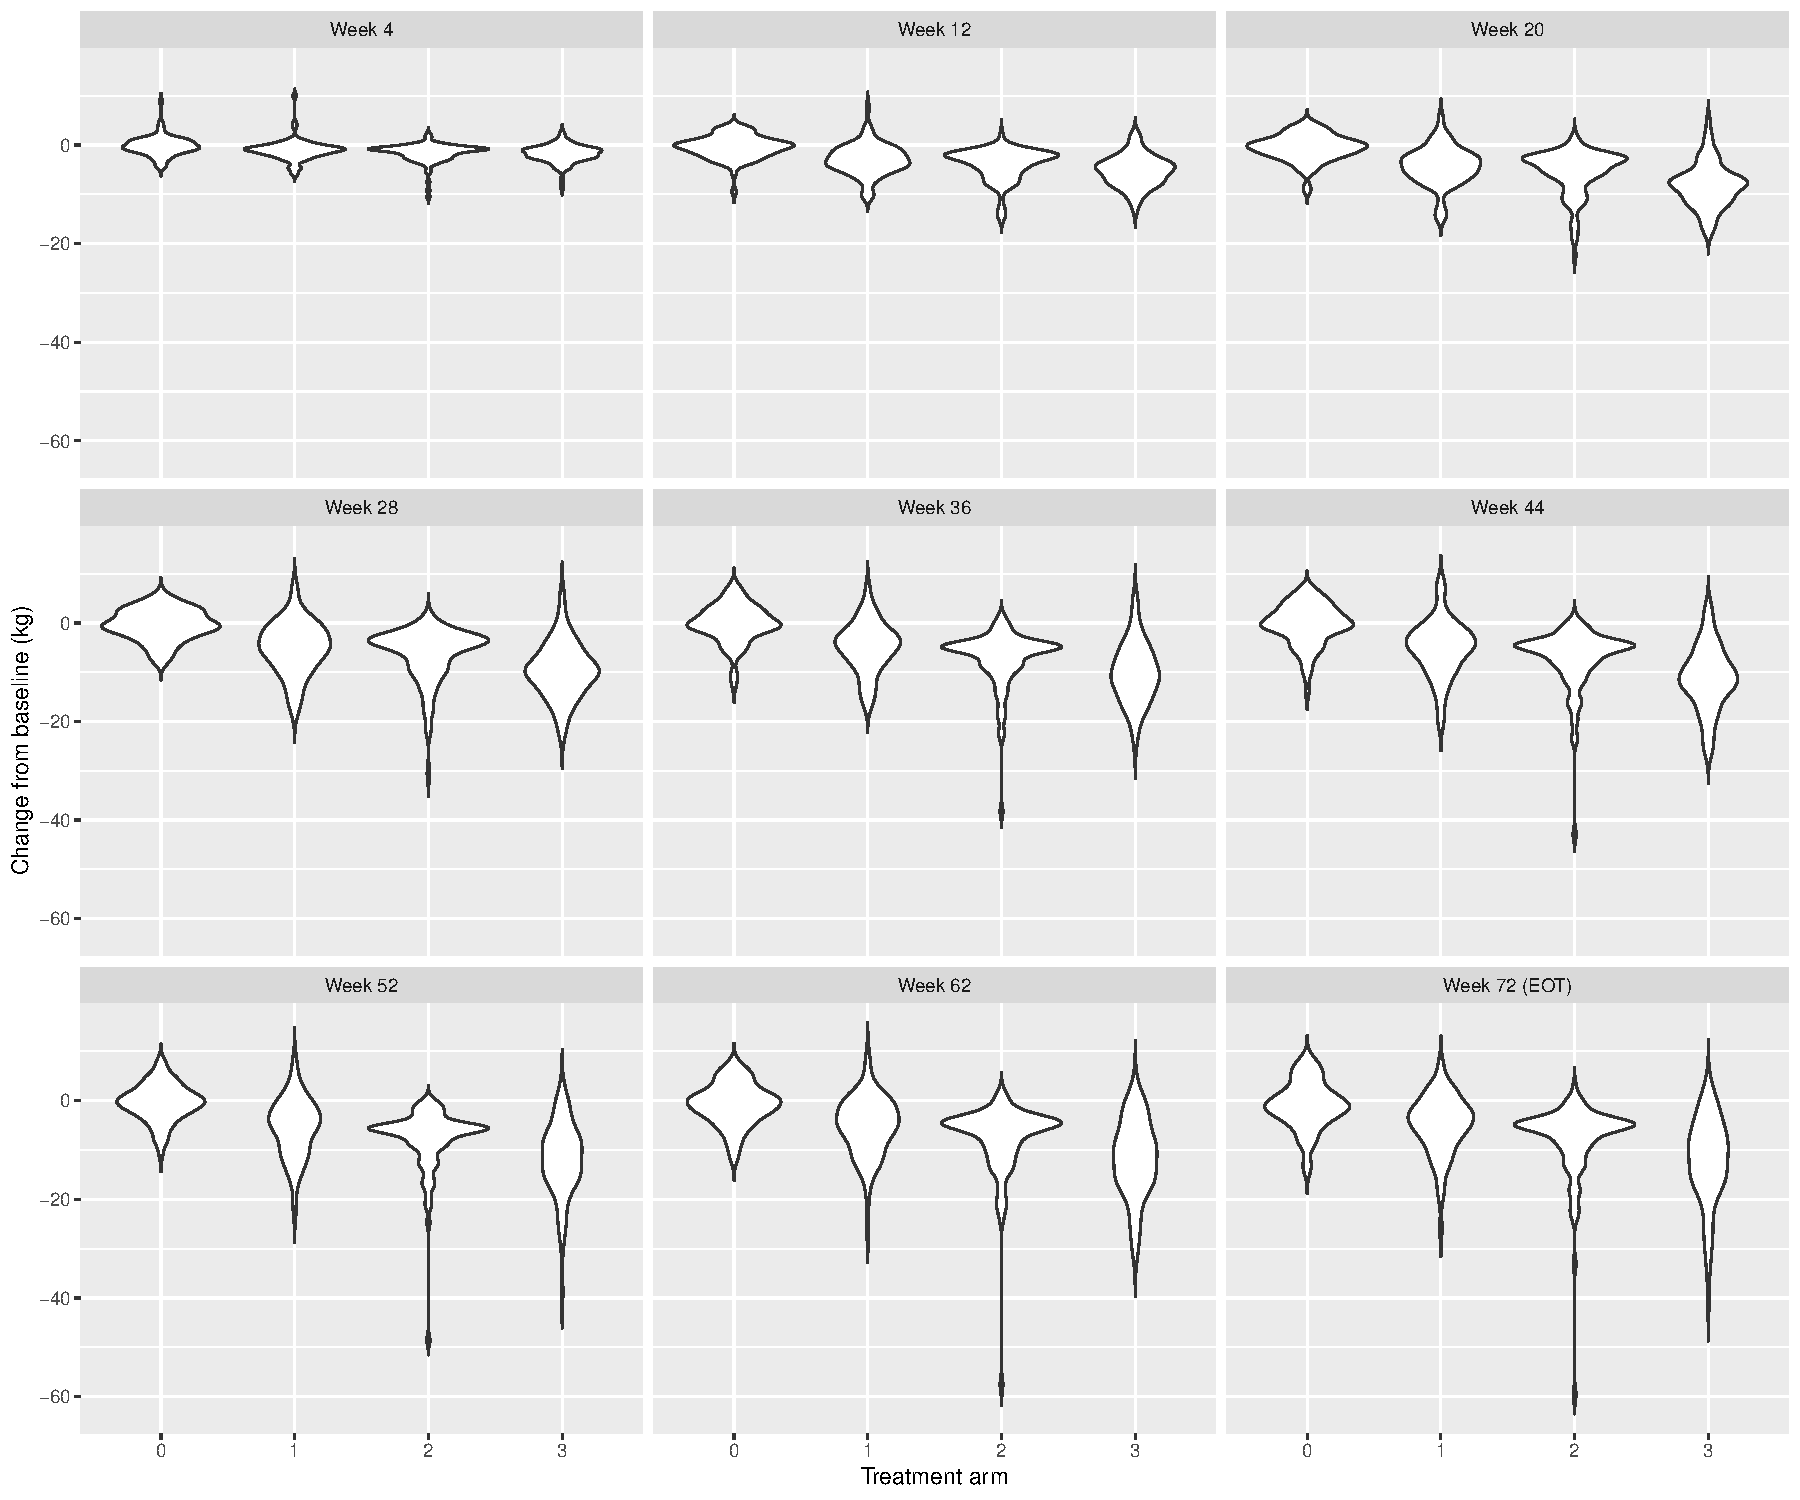
\includegraphics[scale=.55]{violinplot_kg.pdf}
    \caption{Violin plot showing the kernel probability density of weight loss in the four treatment arms at each follow-up visit.}
    \label{fig:my_label}
\end{figure}

%\begin{figure}[h]
%    \centering
%    \includegraphics[scale=.55]{histogram_kg2.pdf}
%    \caption{histograms and density plots of weight loss in the four treatment arms at each %follow-up visit.}
%    \label{fig:my_label}
%\end{figure}



\nocite{*}% Show all bib entries - both cited and uncited; comment this line to view only cited bib entries;
\bibliography{wileyNJD-AMA}%

\clearpage

\end{document}